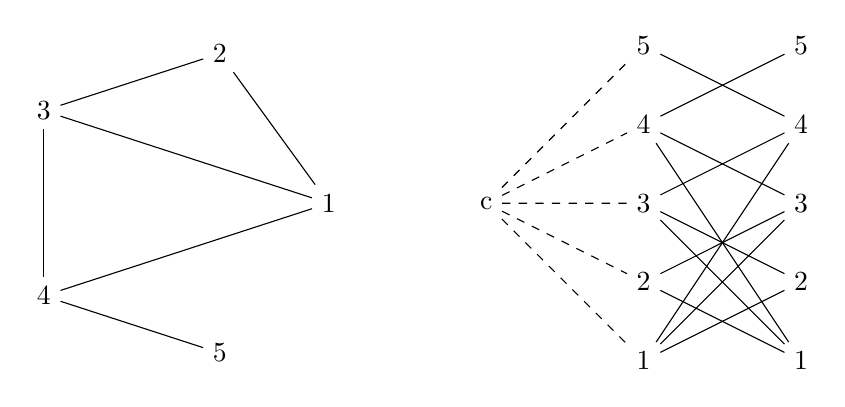
\begin{tikzpicture}[]
\foreach[count=\i] \a in {0,72,...,288}{
	\node(\i) at(\a:2) {\i};
}

\foreach \u \v in {
	1/2,2/3,3/4,4/1,4/5,3/1%
}{
	\draw (\u) -- (\v);
}

\node(c) at(4,0) {c};

\begin{scope}[xshift=6cm, yshift=-3cm]
\foreach \i in {1,...,5}{
	\node(l\i) at(0,\i) {\i};
	\node(r\i) at(2,\i) {\i};
}


\foreach \u \v in {
	1/2,2/3,3/4,4/1,4/5,3/1%
}{
	\draw (l\u) -- (r\v);
	\draw (r\u) -- (l\v);
}

\foreach \i in {1,...,5}{
	\draw[dashed] (c) -- (l\i);
}
\end{scope}
\end{tikzpicture}